\startchapter{The \MonoZll Search}
\label{chapter:prevWork}

This chapter summarizes the previous work done. Section \ref{sec:analysis} gives an overview of the analysis, while Sections \ref{sec:truth} - \ref{sec:code} discuss specific contributions in more detail.

% --------------------------------------------------------------------------------------
\section{Analysis Overview}
\label{sec:analysis}

There are several important aspects of the \monoZ search. The analysis has been repeated fully twice during Run 2, once with the 2015 dataset (3.2 \ifb) and again with the 2015+2016 dataset (36.1 \ifb). The next result will not be ready until the full 2015-2018 Run 2 dataset is collected. The techniques discussed in this section are mainly based on the previous results from the 2015+2016 dataset. 

One of the the first steps of the analysis is to optimize the event selection for the specific signal being considered in the search. A \textit{signal region} must be chosen using some metric that optimizes the amount of signal compared to background. Background events are caused by SM processes that produce the same signature as the dark matter signal. Ideally such processes should be as suppressed as possible in the signal region. Event selections are optimized using Monte Carlo (MC) simulated events for signal and backgrounds. ATLAS MC are sophisticated and include effects from the detector, such as energy resolution. In general, events are selected in order to isolate a \epem or \mpmm pair that have an invariant mass close to the \Z and are recoiling against a sizeable \etmiss vector. The most important kinematic variables are identified and calculated using reconstructed objects as measured in the ATLAS detector (approximate in MC). Additional selection requirements are used to reduce background contributions while attempting to preserve signal. Two signal regions are used in the \monoZ analysis, one where \epem events are selected and the other where \mpmm events are selected. {\color{red}TODO: Maybe list event selections here? Or in appendix?}

Another crucial part of the analysis is in-situ background estimation. Once a signal region has been defined, data can then be used to estimate the dominant backgrounds in that region. When possible it is always preferable to use data instead of MC estimations. This is typically done by defining a control region that has a very high purity in background events, and then somehow transferring the estimate into the signal region. The major backgrounds in the analysis are described below with their percent contribution from the 2015+2016 result. They all emulate the signal by producing $\ell\ell+E_{T}^\text{miss}$. All backgrounds except for the $ZZ$ background are estimated from data.
\begin{enumerate}
	\item	 $ZZ \rightarrow \ell \ell \nu \nu$ (56\%): Dominant, irreducible background. Estimated entirely with MC. 
	\item	 $WZ \rightarrow \ell \nu \ell \ell$ (27\%): Lepton from the $W$ is not reconstructed. 
	\item \Zjets (8\%): Jet(s) are mis-measured as fake \etmiss. 
	\item $WW$, $Wt$, $t\bar{t}$, and $Z\rightarrow \tau \tau$ (8\%): Lepton pair does not come from a \Z.
	\item $W$+jets ($<1\%$): Lepton is misidentified from a jet.
\end{enumerate}

\noindent The data-driven estimation techniques for each of the backgrounds are complex and are not discussed in detail here. Previous work on the estimation of the \Zjets background is discussed ahead.

There are several sources of systematic errors that must be considered in any ATLAS analysis. Experimental systematics come from detector effects, such as the uncertainty in identifying an electron, energy uncertainties due to resolution effects, etc. These systematics are applied to MC samples. Data-driven background estimates will have systematic errors associated with the specific estimation technique. These types of systematics are often the dominant source of systematic uncertainties. Finally, there are theoretical systematics associated with the simulated dark matter signal, including errors from QCD, PDF, and parton showering effects. These will be discussed in more detail in the following section.

\begin{figure}[htb]
\centering
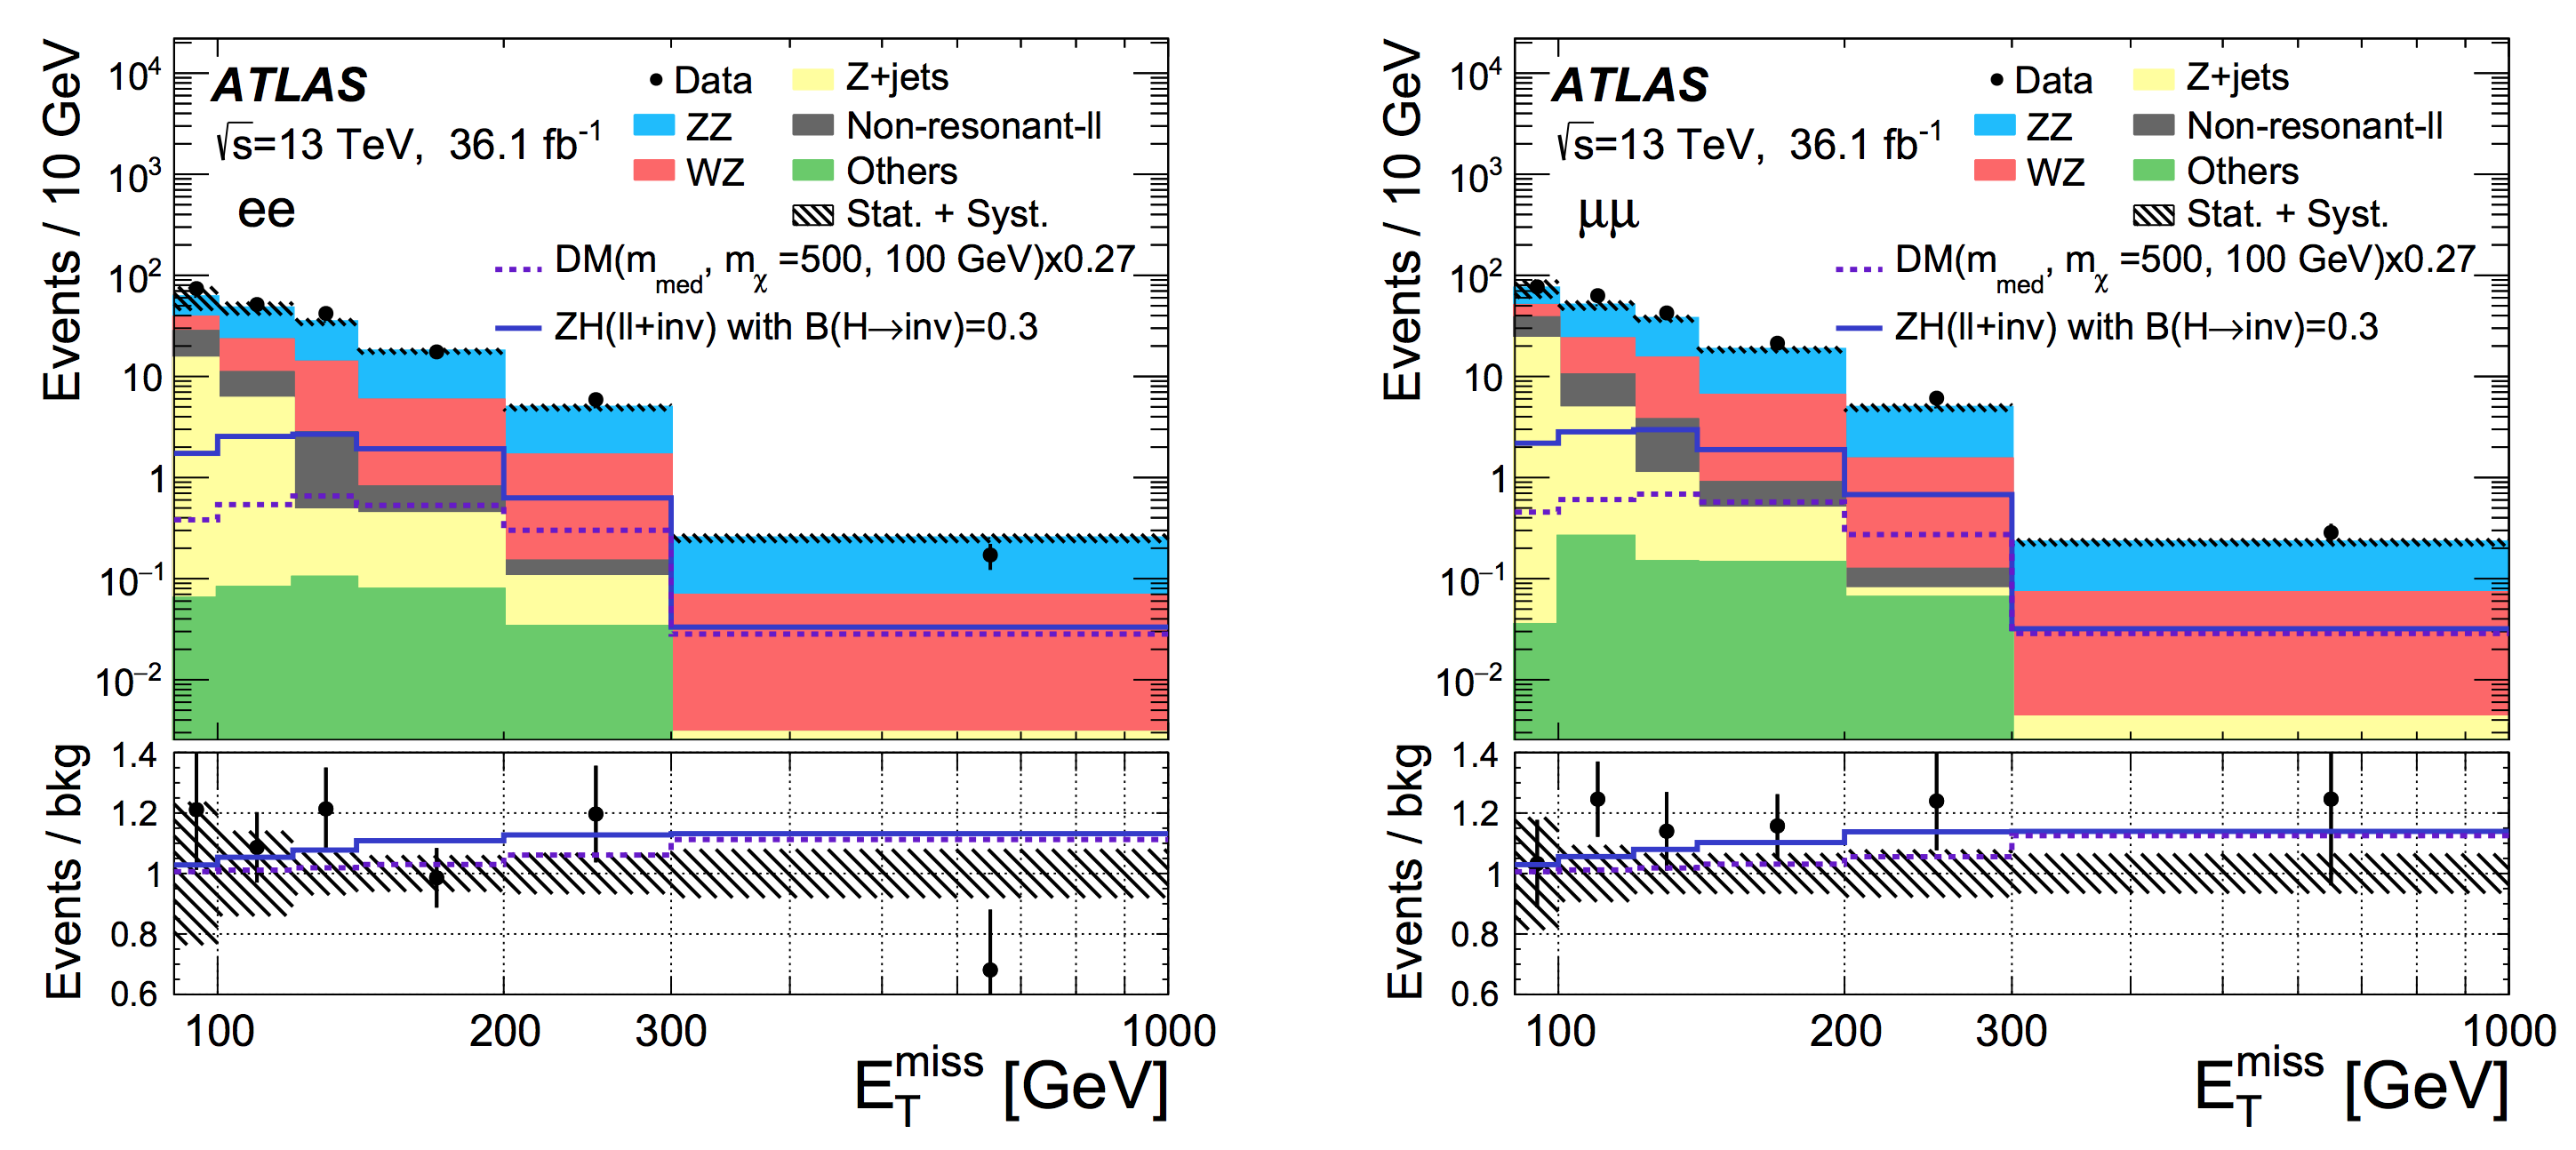
\includegraphics[width=1\textwidth]{Figures/srEPS.png}
\caption{Text}
\label{fig:srEPS}
\end{figure}

After defining a signal region, estimating backgrounds in that signal region, and accounting for the systematic uncertainties of the analysis, the signal region is \textit{unblinded} and the agreement between observed data and expected background estimates is quantified. In the \monoZ analysis the \etmiss is the distribution of interest, where a dark matter signal could manifest. The signal region \etmiss distributions from the 2015+2016 analysis are shown in Figure \ref{fig:srEPS}. If an excess in data is found then there is potential for a discovery. However, as in past iterations of the analysis, if no excess is seen then limits can be set on the dark matter model being studied. This is discussed in detail in the final section of this chapter.

% --------------------------------------------------------------------------------------
\section{Truth Studies} 
\label{sec:truth}

Truth studies are often useful when we want to ignore the effects of the ATLAS detector. \textit{Reconstructed} MC samples include simulation of the detector, whereas \textit{truth-level} MC samples come directly from the MC generator, typically \textsc{MadGraph} \cite{Alwall:2011uj}. Studying these samples allow us to study theoretical effects on the signal. In addition, such samples can be produced quickly and locally, whereas reconstructed samples must undergo heavy duty ATLAS reconstruction which can be computationally intensive. 

A framework has been adapted, called MonoZTruthUVic, for applying truth-equivalent analysis cuts to truth samples. This allows for the analysis to be reproduced at the truth-level. This is useful for several reasons and allows us to estimate how many signal events are theoretically predicted to be in the signal region.

An important study that must be performed at the truth-level is the estimation of theoretical uncertainties on the signal \textit{acceptance}, the number of signal events that end up in the signal regio. There are potentially significant sources of systematic uncertainties from theory that must be considered. It should be noted that systematics from uncertainties in the parton distribution function (PDF) are evaluated in the analysis but are not discussed in detail here. 

The signal acceptance depends on two scales from quantum chromodynamics (QCD) known as the renormalization and factorization scales, $\mu_r$ and $\mu_f$. Both scales are arbitrary and arise from finite order perturbation theory. $\mu_r$ is related to the renormalization of ultraviolet divergences, and $\mu_f$ qualitatively corresponds to the resolution at which the proton is being probed. The cross section for some hard process depends on these scales via

\begin{equation}
\sigma = \int \text{d}x_1 \text{d}x_2 f_1(x_1, \mu_f^2) f_2 (x_2, \mu_f^2) \hat{\sigma}(x_1 p_1, x_2 p_2, \alpha_s(\mu_r), Q^2, \mu_r^2, \mu_f^2),
\end{equation}

\noindent where partons 1 and 2 have PDFs $f_1$ and $f_2$ and momentum fractions $x_1 p_1$ and $x_2 p_2$ respectively. $Q$ is the scale of the hard scatter process determined by the cross section $\hat{\sigma}$.
In short, by simulating dark matter MC with different values for $\mu_f$ and $\mu_r$ and then applying truth-level analysis cuts, the systematic error on the acceptance due to the choice of scales can be quantified. The convention is to generate two variational samples with $\mu_r = \mu_f$, where the scales are doubled in one sample and halved in the other. Then the signal acceptance for both variational samples is calculated and compared to the nominal acceptance. The largest change is taken as the systematic error. This systematic has been observed to be independent of $m_{DM}$, so the errors are evaluated as a function of \mmed. An example of the errors previously used for axial-vector signals is illustrated in Figure \ref{fig:qcd}. These errors are on the order of 1-2\%.

\begin{figure}[htb]
\centering
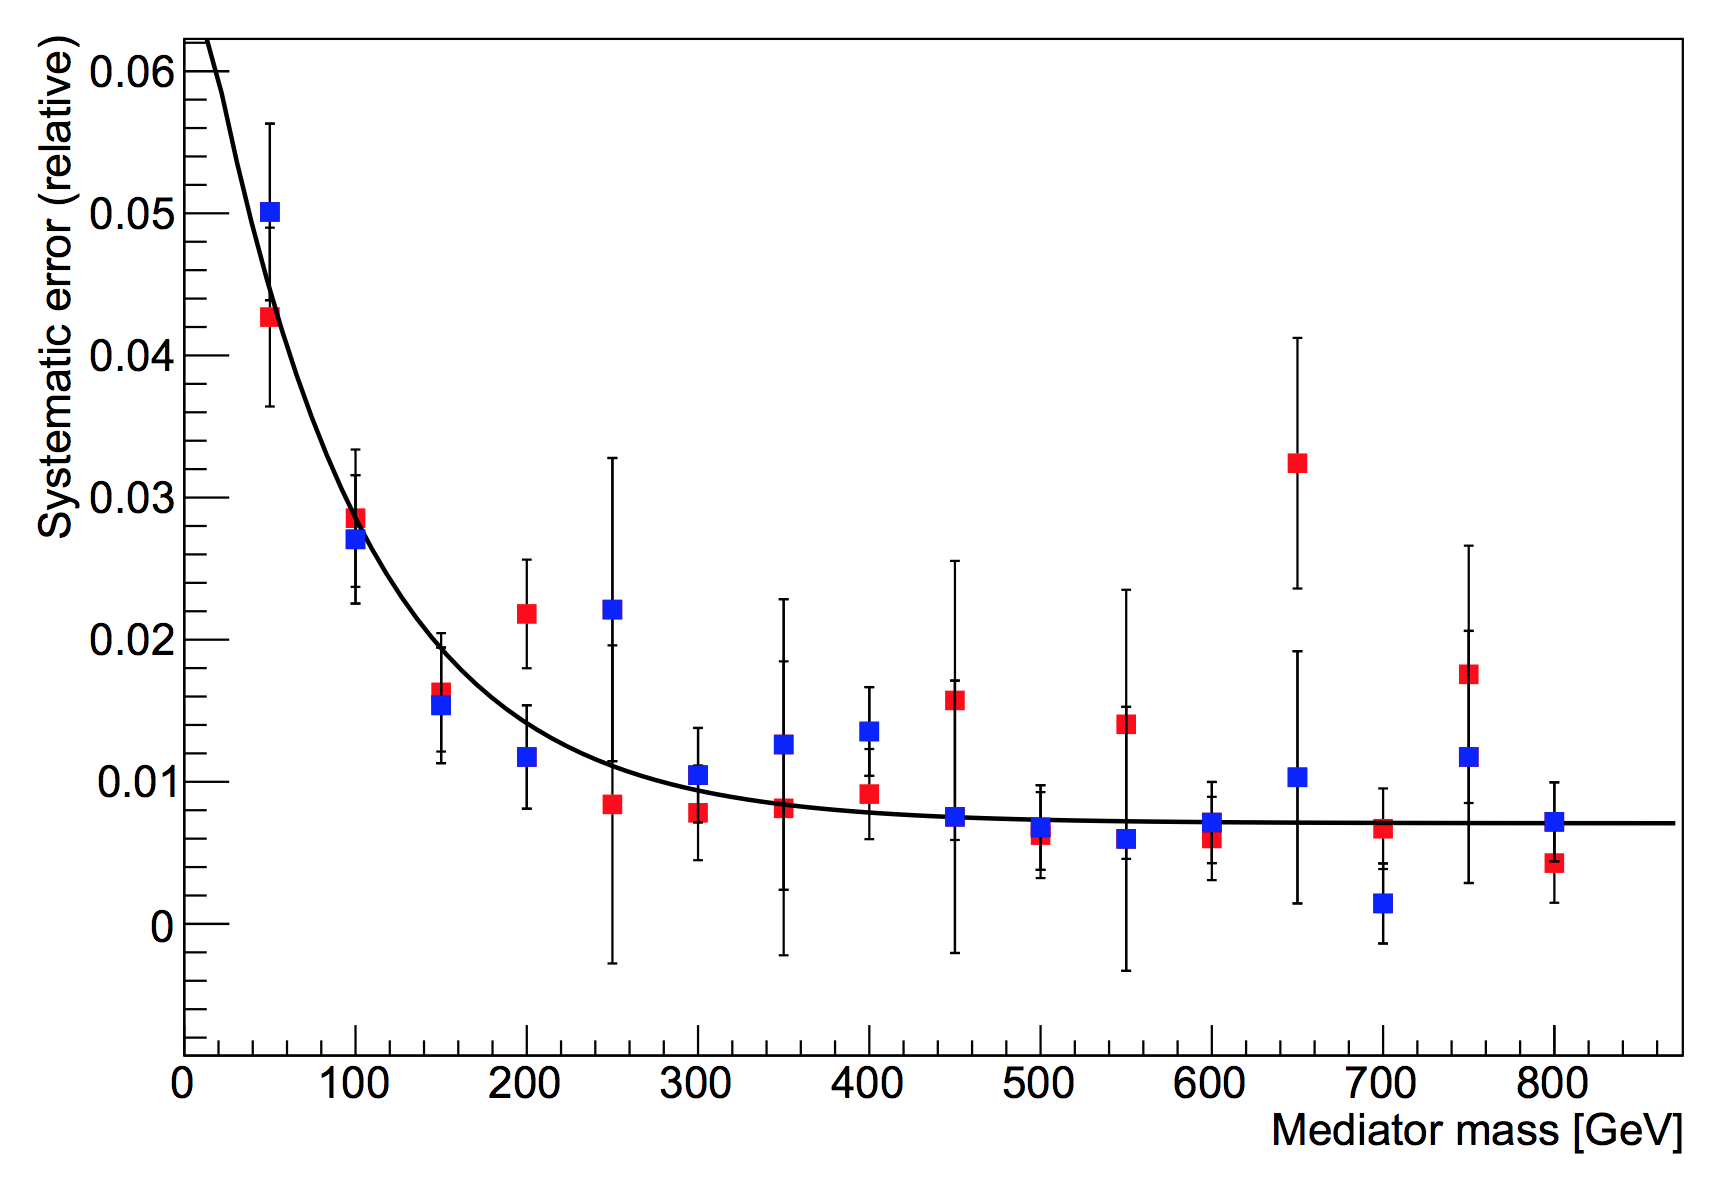
\includegraphics[width=0.5\textwidth]{Figures/qcd.png}
\caption{QCD scale uncertainties as a function of mediator mass for axial-vector signals. Red and blue points correspond to errors obtained from the \ee and \mm signal regions respectively.}
\label{fig:qcd}
\end{figure}

The other source of theoretical uncertainty on the signal acceptance comes from parton showering effects. In the MC samples used by ATLAS, after the hard scatter is simulated it is run through a showering simulator called \pythia \cite{Sjostrand:2014zea}. \pythia adds in several physical effects such as the underlying event (UE), initial and final state radiation (ISR and FSR) of extra jets, and multiple parton interactions (MPI). These are complicated processes governed by QCD and the number of parameters in \pythia that can be set are extensive. To simplify this, ATLAS has a standardized \pythia \textit{tune}, i.e. a set of parameters that serve as the default to be used in MC showering. The signal acceptance depends on the choice of this tune. The uncertainty is evaluated using a prescription whereby ten variations are used to account for each general effect. As for the QCD scale uncertainties, variational MC samples are produced according to each variation, and the difference in the signal acceptance is evaluated compared to the nominal showering. These systematics are typically on the order of 5\%.


% --------------------------------------------------------------------------------------
\section{Estimation of the \Zjets Background}
\label{sec:zjets}

% -------------------------------------------
\subsection{ABCD Method}

\begin{figure}[htb]
\centering
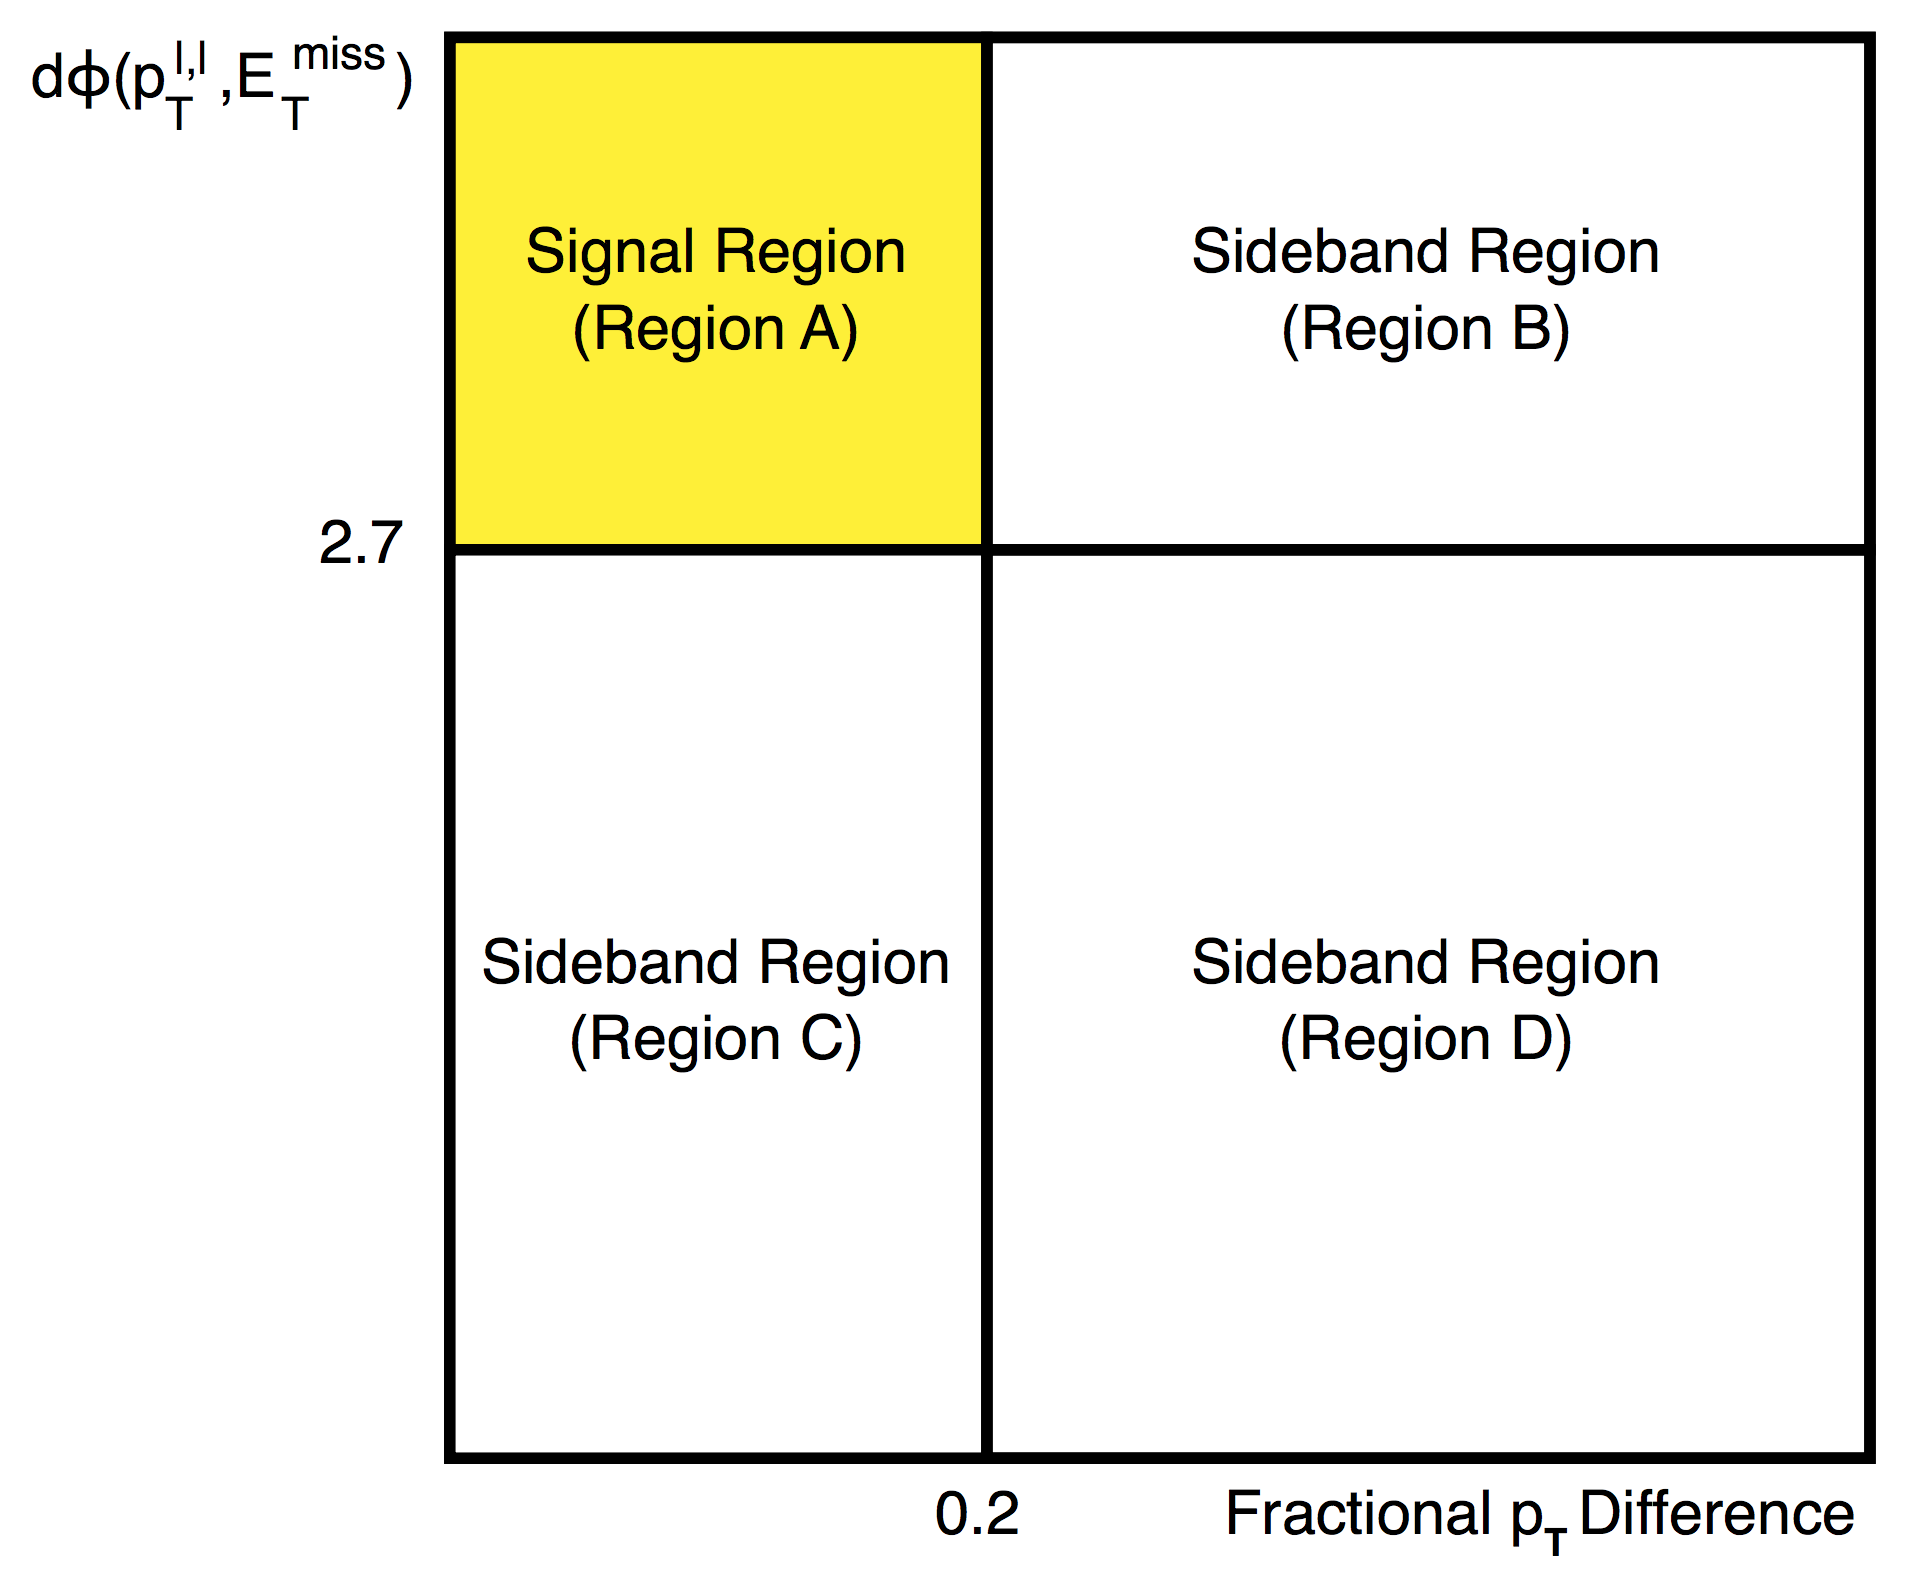
\includegraphics[width=0.5\textwidth]{Figures/abcd2.png}
\caption{Scheme of the ABCD method used with the 2015 dataset.}
\label{fig:abcd}
\end{figure}

One data-driven technique for estimating the \Zjets background is the ABCD method. This was the primary estimation method used for the 2015 result. A schematic of the method is shown in Figure \ref{fig:abcd}. Four regions are defined using two of the kinematic variables from the event selection. This pair of variables is chosen to optimize event statistics in the sideband regions (B, C, and D) and to minimize the correlation between them. Region A is the signal region, the target region that we are trying to estimate the background in. The number of background events in the sidebands are used to estimate the number of background events in A using the assumption that $N_A/N_C = N_B/N_D$. This is true if there is no correlation between the two variables. Then the number of \Zjets events in A is given by:

\begin{equation}
N_\text{A}^\text{est} = N_\text{C}^\text{obs,corr} \times \frac{N_\text{B}^\text{obs,corr}}{N_\text{D}^\text{obs,corr}}
\end{equation}

\noindent $N_\text{B}$, $N_\text{C}$, and $N_\text{D}$ are the observed number of events in each sideband control region with non-\Zjets events subtracted (using MC).

The main challenges for this method come from having correlations between the two variables and having enough statistics in data in all of the sidebands. The validity of this technique is evaluated by looking at the agreement between the three ratios $N_\text{A}/N_\text{C}$ (MC), $N_\text{B}/N_\text{D}$ (MC), and $N_\text{B}/N_\text{D}$ (data). If the method works perfectly then these ratios will agree. In addition, the agreement of these ratios should agree as the other event selections are applied. However, correlations cause deviations in the agreement, and low statistics in one or more of the sidebands can lead to large errors on the ratios after all selections are applied. And, if the ratios change with other selections, this suggests more complicated correlations with other variables that enhance the correlation between the two variables used for the method. These effects are all taken into account with systematic errors that are evaluated to be about $\pm$70\% on the \Zjets estimate. These turned out to be dominant uncertainties in the analysis for the 2015 result.

% -------------------------------------------
\subsection{\gjets Technique}
\label{sec:gjets}

The \Zjets estimation had to be modified for the 2015+2016 result. The event selection was reoptimized and introduced new variables, and correlations had a more pronounced effect in the ABCD method. Because of this, a second technique was developed alongside a modified ABCD method. The technique is known as the \gjets reweighting method. The theory is described in \cite{Ask:2011xf} and the application has been adapted from an ATLAS SUSY search \cite{Galster:2151990}.

The \gjets method uses events with a photon and jets to estimate the fake \etmiss in \Zjets events. \gjets event topologies are similar to \Zjets events as they both consist of a well-measured \Z or photon recoiling against jets, and the \etmiss arises from jet mis-measurements. However there are some kinematic differences that need to be accounted for. This is done by reweighting the \gjets MC events to transport them to \Zjets MC events. Typically the \pt distribution of the photon is scaled to match the \pt distribution of the \Z (i.e. the \pt of the two leptons). The multiplicative factor needed to scale each \pt bin is used as an event weight for the \gjets events: 

\begin{equation}
w(p_\text{T}^\gamma) = \frac{N_{Z\text{+jets}}(p_\text{T}^{\ell\ell})}{N_{\gamma\text{+jets}}(p_\text{T}^\gamma)}
\end{equation}

\noindent After the reweighting the \etmiss distribution for the \gjets events improves to match the \Zjets events (most obviously the tail increases at high \etmiss). The reweighting is applied fairly early in the event selection and then subsequent selections are applied; the agreement between \gjets and \Zjets events is monitored down to the signal region. Once reliable agreement is seen, then the method can be performed using data instead of MC.

In the \monoZ analysis, \pt reweighting was not sufficient to have good agreement between \gjets and \Zjets events. Two approaches were taken in an attempt to rectify the remaining differences. The first is a photon smearing method as used in \cite{Galster:2151990}. This is done by looking at the component of the \etmiss along the \Z/photon direction, \etmisspar. The idea is that any difference in \etmisspar between \Zjets and \gjets events comes from lepton mis-measurements in the \Zjets events, leading to a larger \Z resolution compared to the photon. Hence the photon \pt and \etmisspar can be smeared to match the \Z resolution. This procedure was carried out in the \monoZ analysis but minimal improvements were seen because the photon and \Z were observed to have very similar resolutions. Therefore a second reweighting scheme was adapted to improve the agreement in the \etmiss distributions. Instead of only reweighting by \pt, a secondary reweighting is applied using another variable. Several variables were investigated; in the end \etmissht gave the best results ($H_T$ = scalar sum of lepton \pt and jet \pt). In addition, the reweighting could be applied using 2D weights or with two 1D (2x1D) weights. The 2D reweightings that were investigated gave the best \etmiss agreement, but the weights were unreliable due to limited statistics (e.g. weights in \pt and \etmissht bins). 2x1D reweighting schemes were also studied. Here an added complication is that the two variables that are reweighted are treated as uncorrelated, whereas for 2D reweighting the correlation is accounted for automatically. So in a 2x1D scheme, when reweighting the second variable, if the previously reweighted \pt distribution does not change, then the variables can be treated uncorrelated. This was seen in \pt and \etmissht. Also the weights with 2x1D schemes were observed to be far more reliable because of the higher statistics use in the weight calculation. This was further tested by splitting the \gjets MC into two statistically independent halves; one half was used to obtain the weights and the other half had them applied. The agreement between both reweighted halves of the \gjets sample was excellent. 

\begin{figure}[h]
\centering
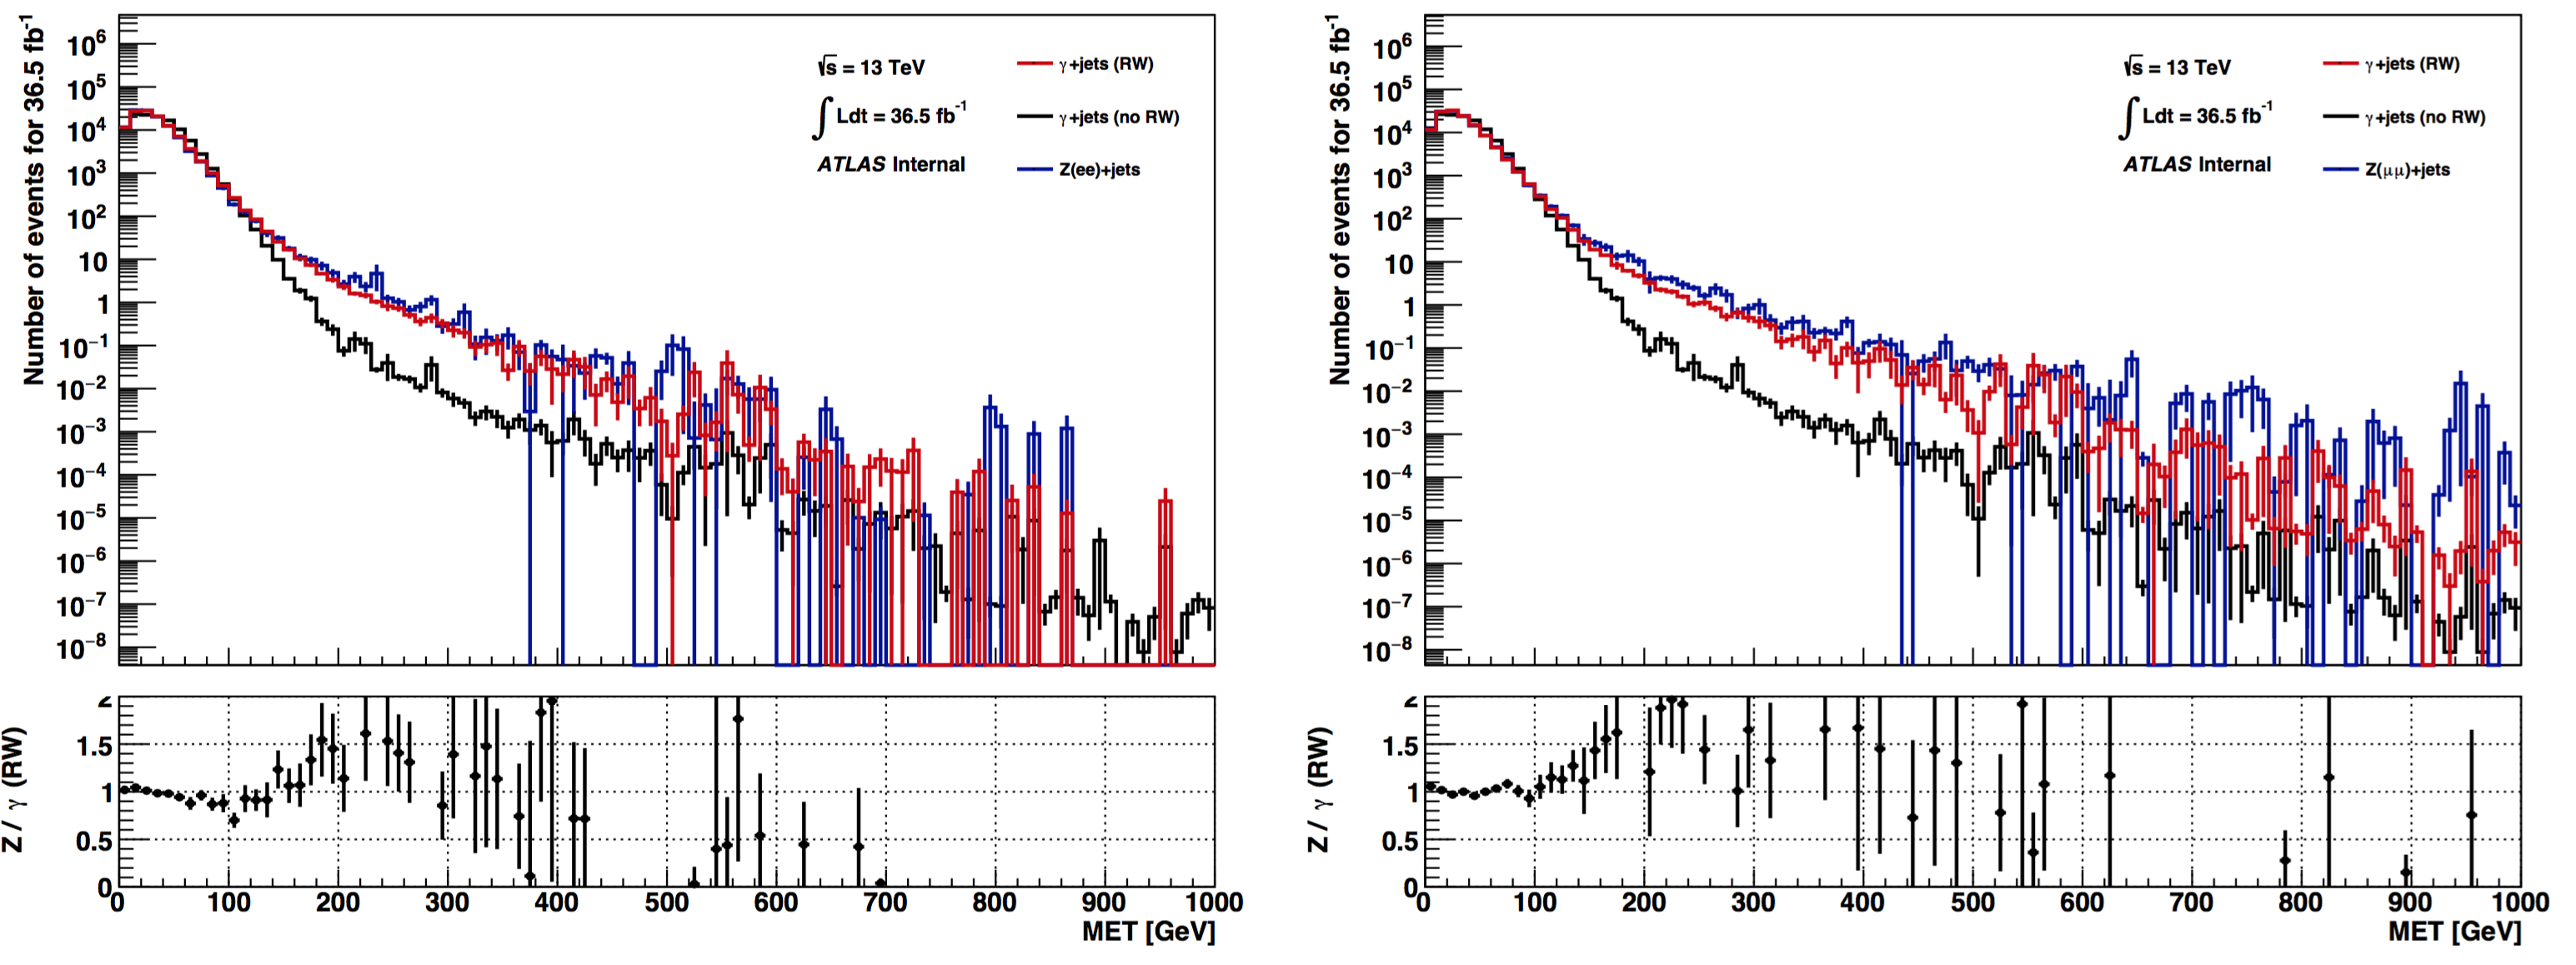
\includegraphics[width=1\textwidth]{Figures/gjets.png}
% EPS paper: https://arxiv.org/abs/1708.09624
\caption{\etmiss distributions for \gjets events (red) and \Zjets events (black without reweighting, blue with reweighting).}
\label{fig:gjets}
\end{figure}

Due to time constraints in the analysis for the 2015+2016 result, the development of this technique is still under development and has yet to be tested on data. In the end a 2x1D reweighting scheme using \pt and \etmissht gave the best results in MC. Figure \ref{fig:gjets} shows the \etmiss distributions for \Zjets and reweighted \gjets events (at an early selection step). From \Zjets MC, the predicted yield in the \ee and \mm signal regions is approximately $0.45 \pm 0.90$ events. The best observed reweighted \gjets prediction is $2.0 \pm 0.1$. The results nearly agree within statistical errors, but differences are still observed in the \etmiss tail. Since this is the region of interest in the \monoZ search, care must be taken to study these differences and quantify the systematic errors from the reweighting technique. The next steps to developing and improving the \gjets technique are discussed in the next chapter.

% --------------------------------------------------------------------------------------
\section{Dark Matter Limit Setting}
\label{sec:limits}

In the case that no excess is observed in data, upper limits are set on the signal strength for each of the dark matter models. These are then translated into limits on the masses of the dark matter particles, \mchi and \mmed. Hypothesis tests are performed using the \histfitter \cite{Baak:2014wma} framework. The signal region \etmiss distributions are inputted to \histfitter for data, expected signal and backgrounds, and all systematic uncertainty variations. \histfitter is then used to calculate upper limits on the amount of signal using the CL$_{s}$ method \cite{Cowan:2010js}, a standard in the ATLAS experiment. 

The statistical analysis of the data uses a binned likelihood function constructed as:
\begin{equation}
L(\mu,\boldsymbol{\theta}) = \prod_{i=1}^N \frac{(\mu s_i + b_i)^{n_i}}{n_i !} e^{-(\mu s_i + b_i)} \times \prod_{j=1}^M G(\theta_j^0, \theta_j)
\label{eqn:likelihood}
\end{equation}

\noindent The first term is the product of Poisson probabilities to observe $n_i$ events for each signal region bin $i$ that has $\mu s_i + b_i$ expected events. $s_i$ and $b_i$ are the predicted signal and background yields in each bin, and $\mu$ is the signal strength parameter (also called the \textit{parameter of interest}). $\mu=0$ is the background-only hypothesis, and $\mu=1$ is the signal+background hypothesis. The dependence of the signal and background predictions on the systematic uncertainties is described by a set of nuisance parameters (NPs) $\vec{\theta}$ (= $\boldsymbol{\theta}$), which are each parametrized by a Gaussian. The second term in Equation \ref{eqn:likelihood} is a product of these terms over all systematics, where $\theta_j^0$ is the measured central value around which $\theta_j$ varies. In \histfitter the $G$'s are parametrized so that each $\theta_j^0$ is fixed to 0 with standard deviation = 1.

The nominal fit result is obtained by maximizing the likelihood function with respect to all parameters. This is referred to as the maximum likelihood, $L(\hat{\mu}, \hat{\boldsymbol{\theta}})$, where $\hat\mu$ and $\hat{\boldsymbol{\theta}}$ are the parameters that maximize the likelihood. A \textit{test statistic}, $\tilde q_\mu$, is then constructed based on the profile likelihood ratio $\lambda(\mu)$:

\begin{equation}
\lambda(\mu) = \frac{L(\mu, \hat{\hat{\boldsymbol{\theta}}})}{L(\hat{\mu}, \hat{\boldsymbol{\theta}})}
\label{eqn:proflike}
\end{equation}

\noindent $\hat{\hat{\boldsymbol{\theta}}}$ are the NP values that maximize the likelihood for a fixed $\mu$. Because the denominator is the maximum likelihood, it must be true that $0 \leq \lambda(\mu) \leq 1$. Hence smaller values of $\lambda(\mu)$ indicate less agreement between the measured $\hat{\mu}$ and the hypothesized $\mu$. For the test statistic $\tilde q_\mu$, larger values are interpreted as greater incompatibility between measurement and the $\mu$ hypothesis. The corresponding p-value, $p_\mu$, is then defined as:

\begin{equation}
p_\mu = \int_{\tilde{q}_{\mu,\text{obs}}}^\infty f(\tilde{q}_\mu | \mu) \text{d}\tilde{q}_\mu
\label{eqn:pmu}
\end{equation}

\noindent Here $f(\tilde{q}_\mu | \mu)$ is the probability density function of $\tilde{q}_\mu$ assuming the $\mu$ hypothesis, and $\tilde{q}_{\mu,\text{obs}}$ is the value of $\tilde{q}_\mu$ computed for the observed data.
Asymptotic formulae \cite{Cowan:2010js} are used to calculate the closed form of $f(\tilde{q}_\mu | \mu)$. $p_\mu$ can also be written as:

\begin{equation}
p_\mu \equiv p_{s+b} = P(\tilde q_\mu \geq \tilde{q}_{\mu,\text{obs}} | s+b)
\end{equation}

\noindent Hence it is the probability to observe a test statistic greater than or equal to the observed value, given that the $s+b$ ($\mu=1$) hypothesis is true. Performing exclusion tests with $p_{s+b}$ is known as the CL$_{s+b}$ method. This analysis uses the CL$_s$ method, where the p-value, or the ``CL$_s$ value,'' is defined as:

\begin{equation}
\text{CL}_s \equiv \frac{p_{s+b}}{1-p_b},
\end{equation}

\noindent where 

\begin{equation}
p_b = P(\tilde q_\mu \leq \tilde{q}_{\mu,\text{obs}} | b).
\end{equation}

Using the CL$_s$ method, any $\mu$ values that give CL$_s<0.05$ are excluded at the 95\% confidence level (CL). These upper limits on $\mu$ are then extracted from \histfitter, and dark matter mass exclusion limits are produced using the MonoZLimitsUVic framework that was written for this purpose.

Figure \ref{fig:limits} shows the exclusion limits from the 2015+2016 result on \mchi vs \mmed for axial-vector and vector mediators from the LO simplified models. The mass region inside the contour is excluded at the 95\% CL. The relic density line indicates where the particles and interactions of the model are by themselves sufficient for explaining the observed DM abundance in the universe.

\begin{figure}[htb]
    \centering
    \begin{subfigure}[b]{0.48\textwidth}
        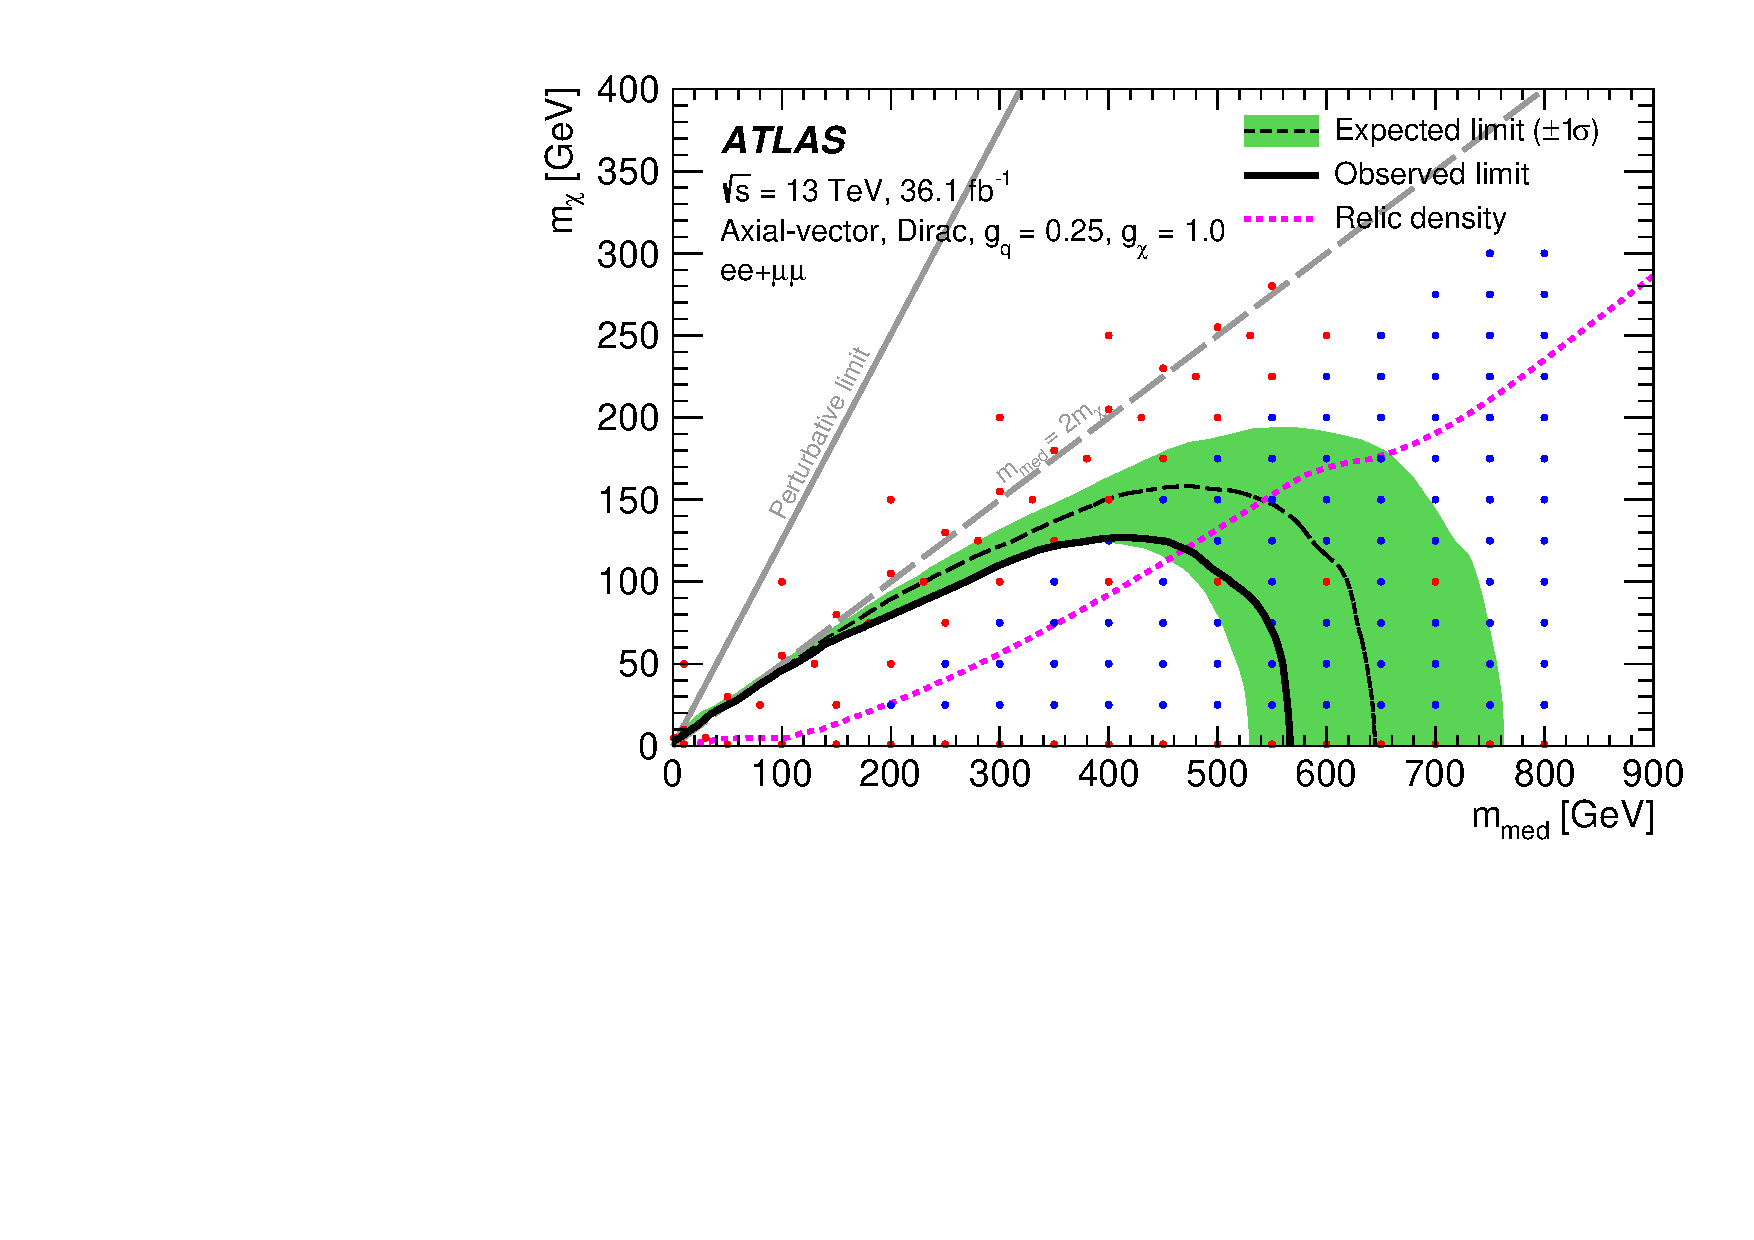
\includegraphics[width=\textwidth]{Figures/limits_dmA.pdf}
        \label{fig:limits_dmA}
    \end{subfigure}
    ~ %add desired spacing between images, e. g. ~, \quad, \qquad, \hfill etc. 
      %(or a blank line to force the subfigure onto a new line)
    \begin{subfigure}[b]{0.48\textwidth}
        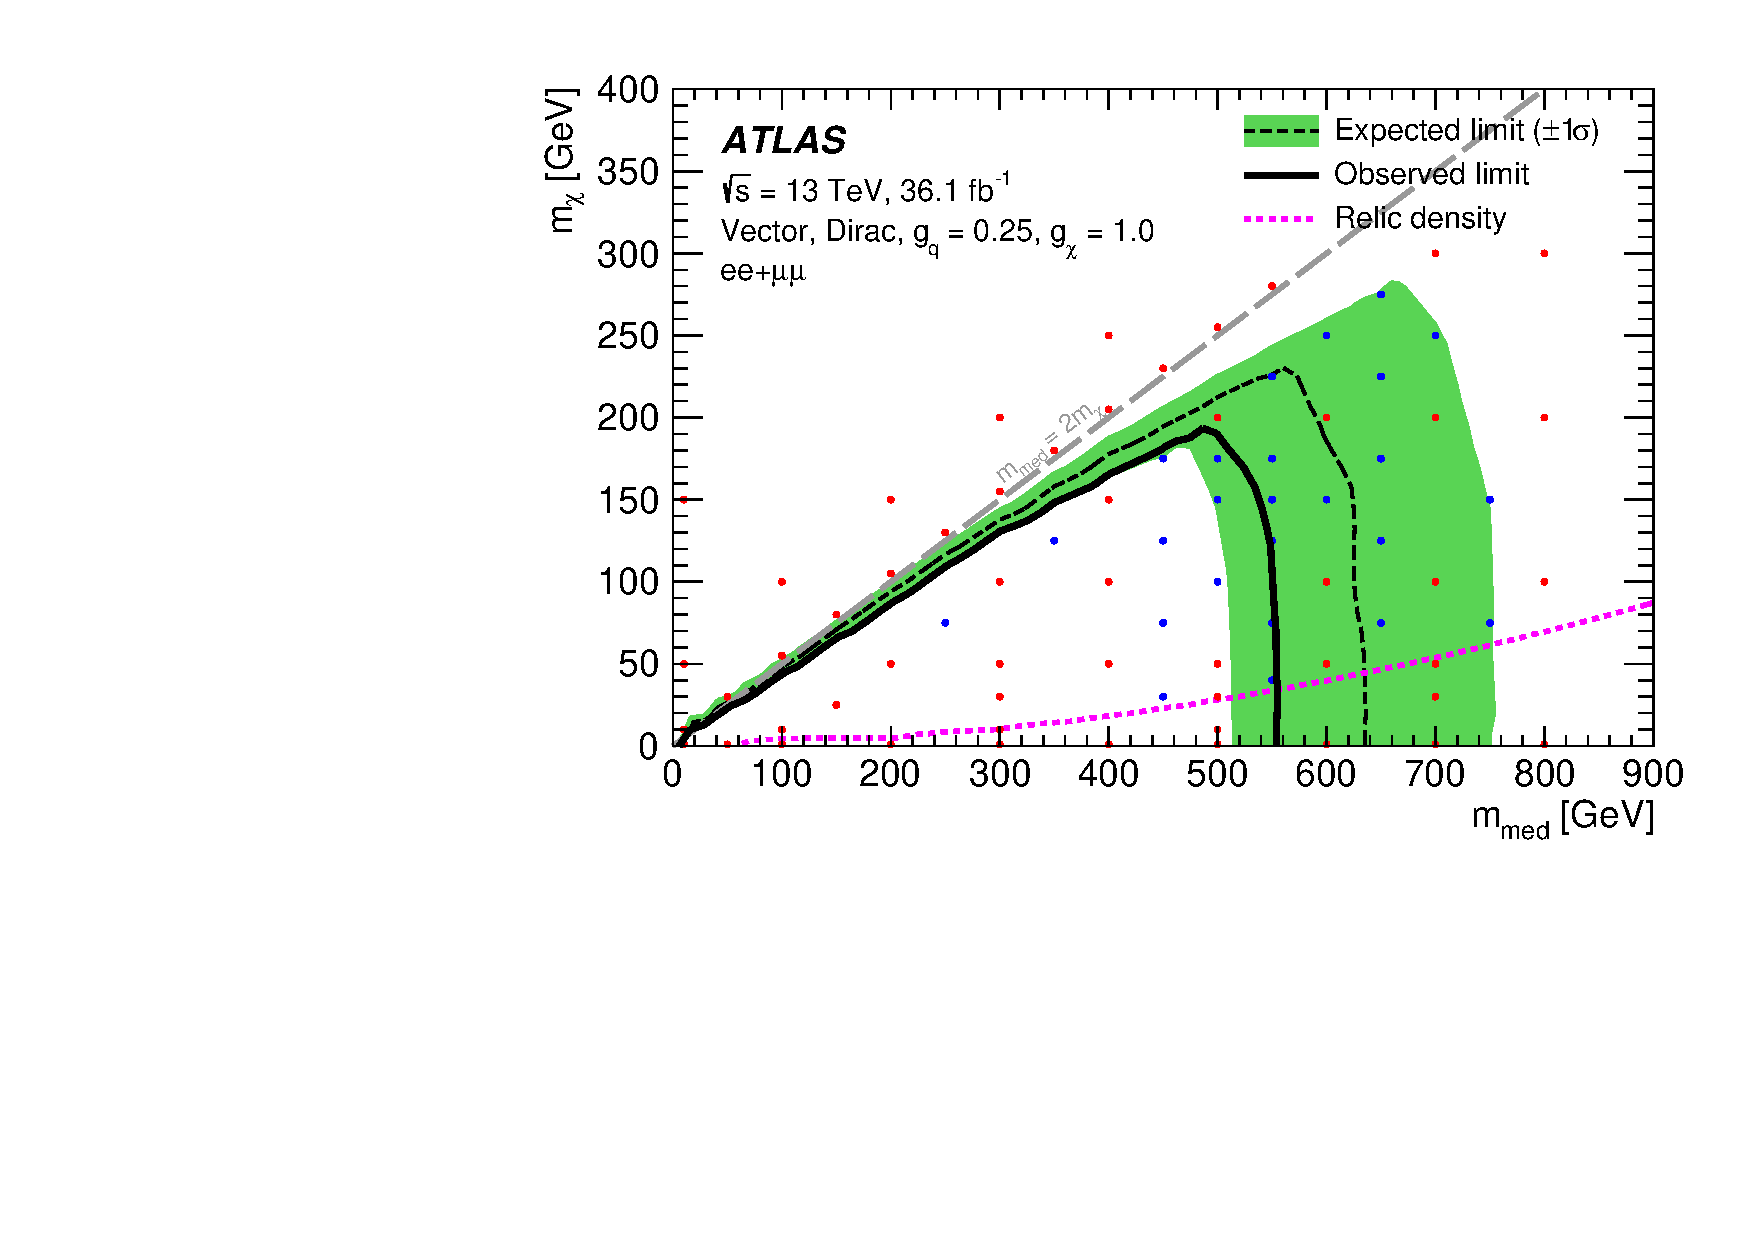
\includegraphics[width=\textwidth]{Figures/limits_dmV.pdf}
        \label{fig:limits_dmV}
    \end{subfigure}
    \caption{Axial-vector (left) and vector (right) exclusion limits on \mchi vs \mmed with 36.1 \ifb.}
\label{fig:limits}
\end{figure}

The 2D mass limits have also been recast into limits on the DM-proton scattering cross section for comparison with DD experiments. The procedure for doing so is given in \cite{Boveia:2016mrp}. Figure \ref{fig:xsec} shows the recast \monoZ limits for the spin-dependent (SD) and spin-independent (SI) scattering cross sections vs \mmed. The cross section is SD if the isotope used in the DD experiment has an unpaired proton or neutron. The limits shown are at the 90\% CL in accordance with the standard used by DD experiments. The coloured lines overlaid are limits set by DD experiments.

\begin{figure}[htb]
    \centering
    \begin{subfigure}[b]{0.48\textwidth}
        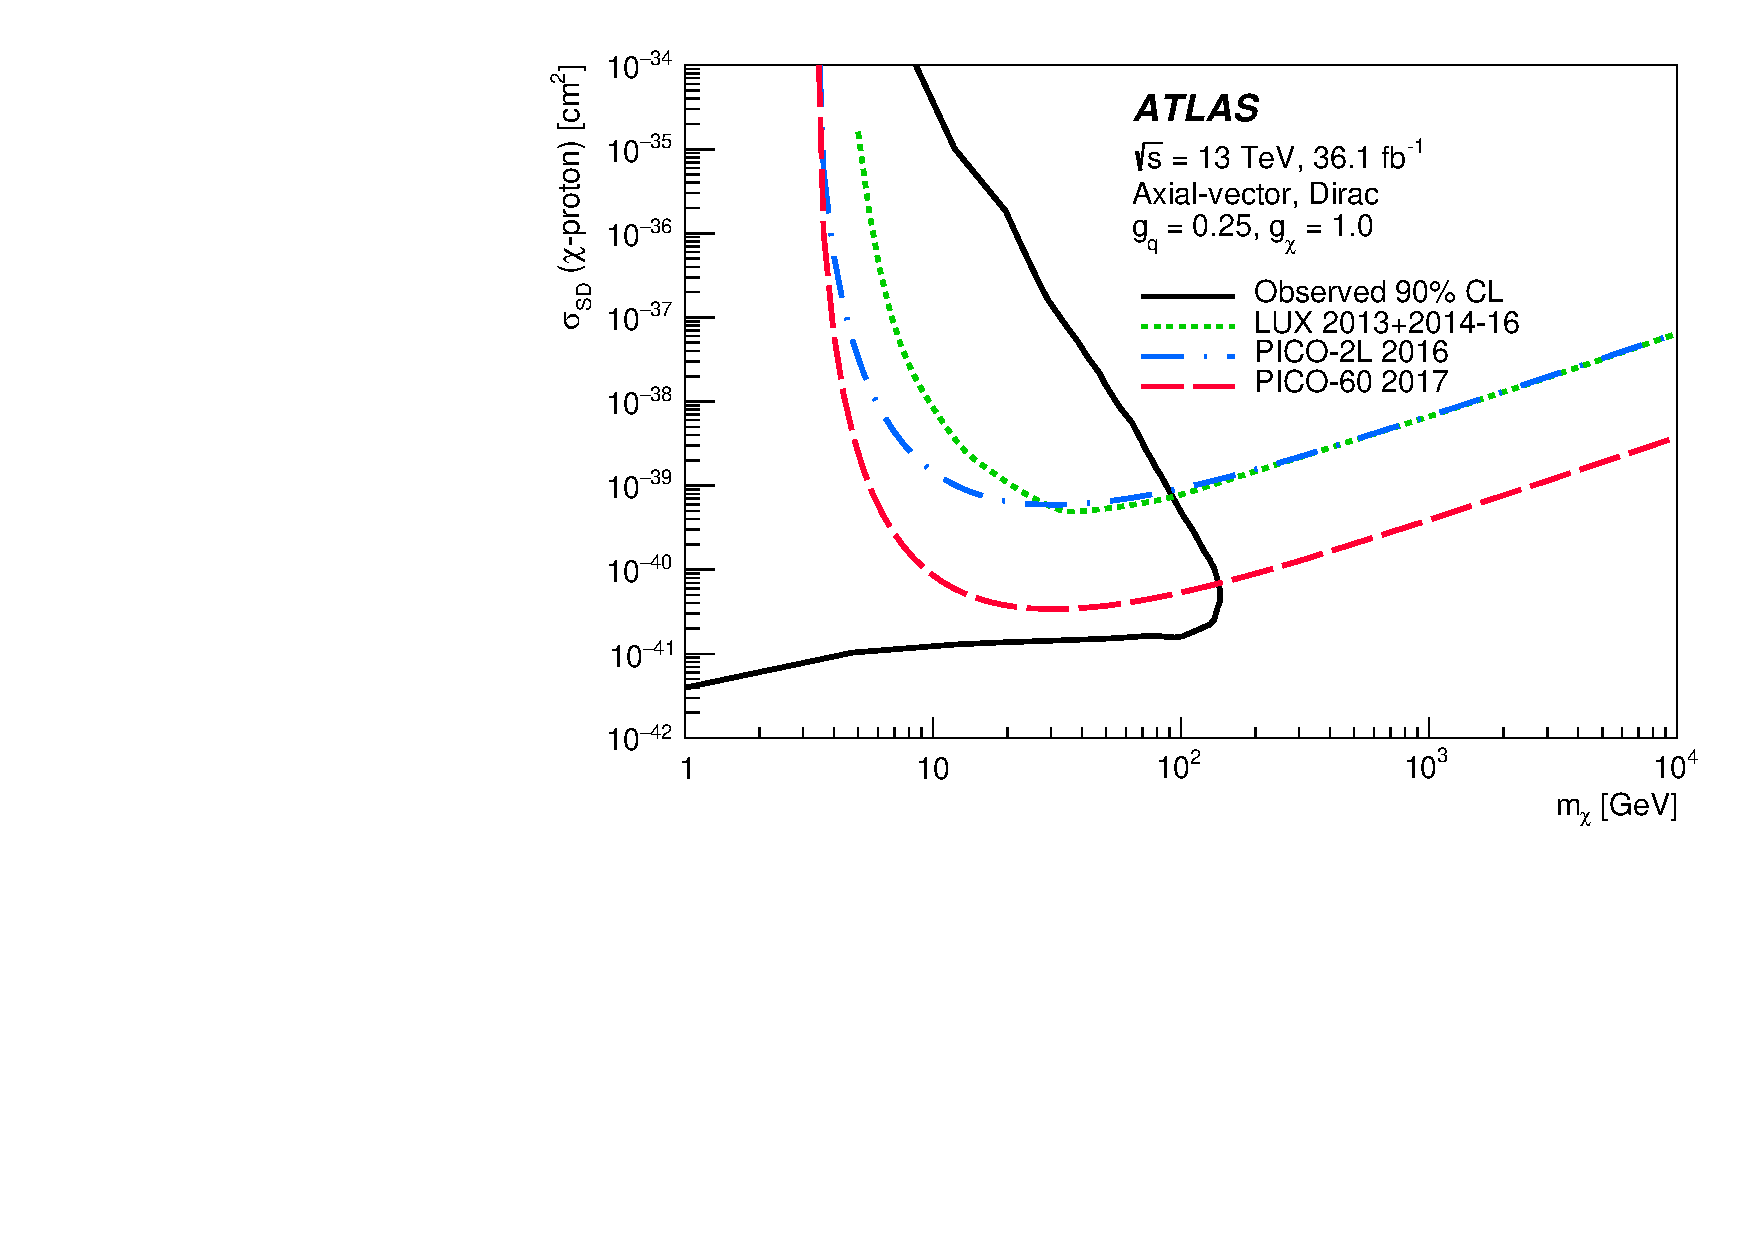
\includegraphics[width=\textwidth]{Figures/xsec_dmA.pdf}
        \label{fig:xsec_dmA}
    \end{subfigure}
    ~ %add desired spacing between images, e. g. ~, \quad, \qquad, \hfill etc. 
      %(or a blank line to force the subfigure onto a new line)
    \begin{subfigure}[b]{0.48\textwidth}
        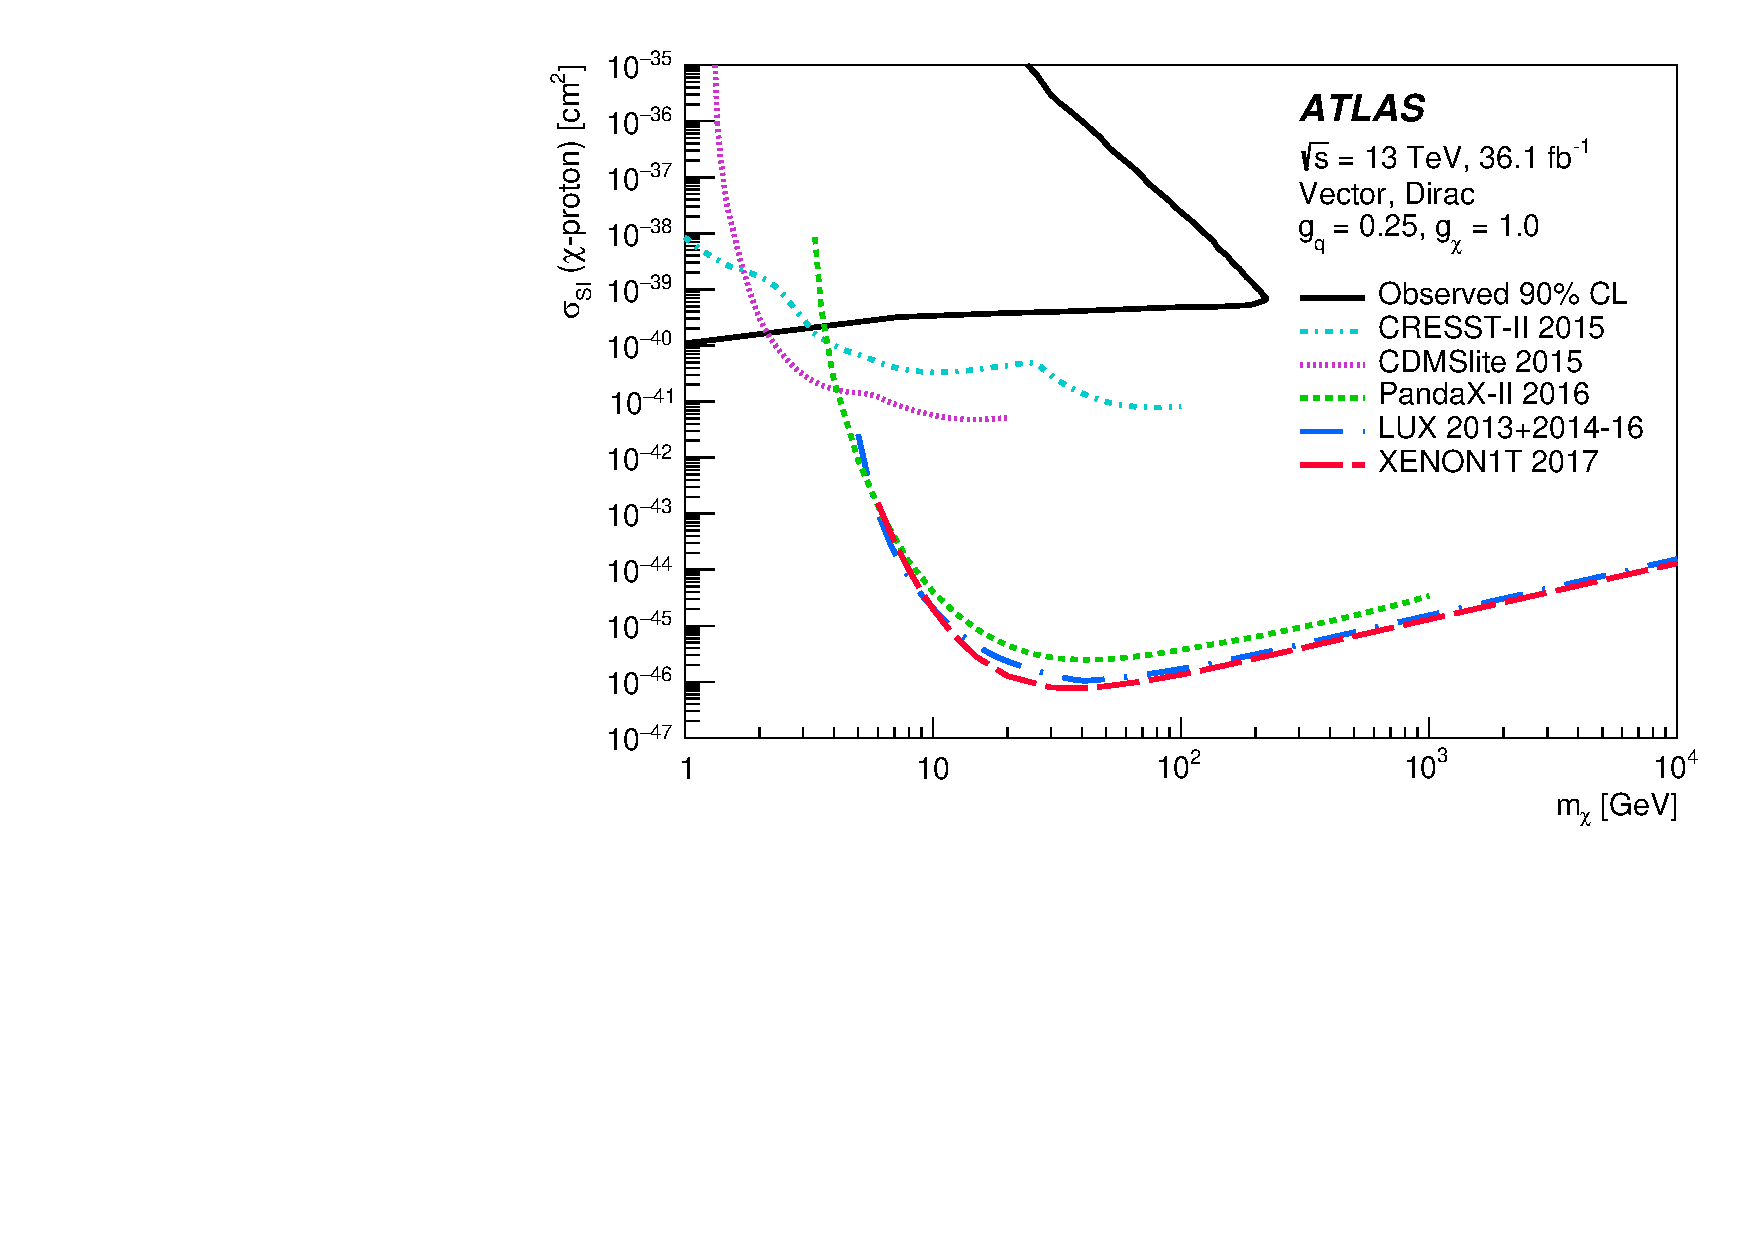
\includegraphics[width=\textwidth]{Figures/xsec_dmV.pdf}
        \label{fig:xsec_dmV}
    \end{subfigure}
    \caption{Axial-vector (left) and vector (right) exclusion limits on the DM-nucleon scattering cross section vs \mmed with 36.1 \ifb.}
\label{fig:xsec}
\end{figure}

Exclusion limits on the 2HDM+PS model have also been set with the 2015+2016 dataset. These are shown in Figure \ref{fig:2hdma}. Limits are set on $m_H$ vs $m_a$ as well as $\tan(\beta)$ vs $m_a$.

\begin{figure}[htb]
    \centering
    \begin{subfigure}[b]{0.48\textwidth}
        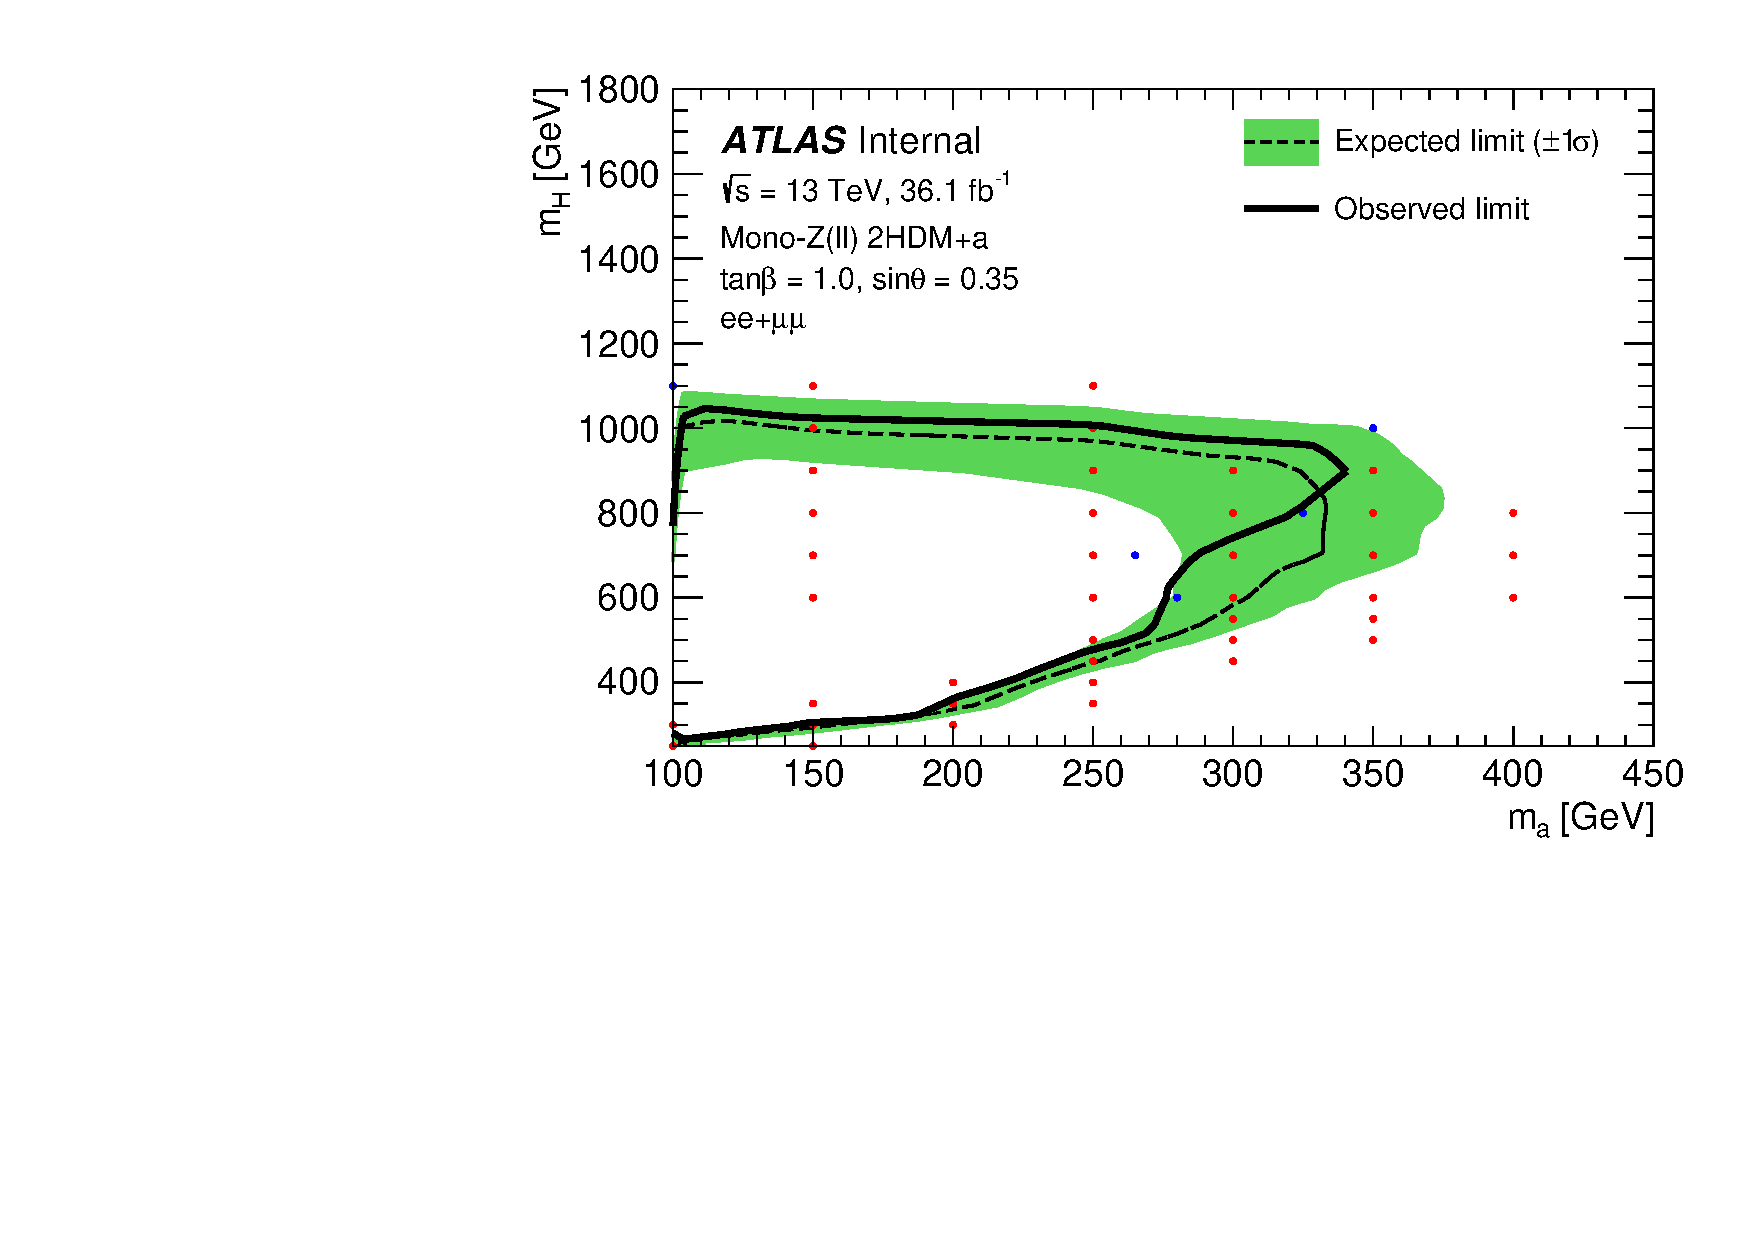
\includegraphics[width=\textwidth]{Figures/limits_2hdma.pdf}
        \label{fig:limits_2hdma}
    \end{subfigure}
    ~ %add desired spacing between images, e. g. ~, \quad, \qquad, \hfill etc. 
      %(or a blank line to force the subfigure onto a new line)
    \begin{subfigure}[b]{0.48\textwidth}
        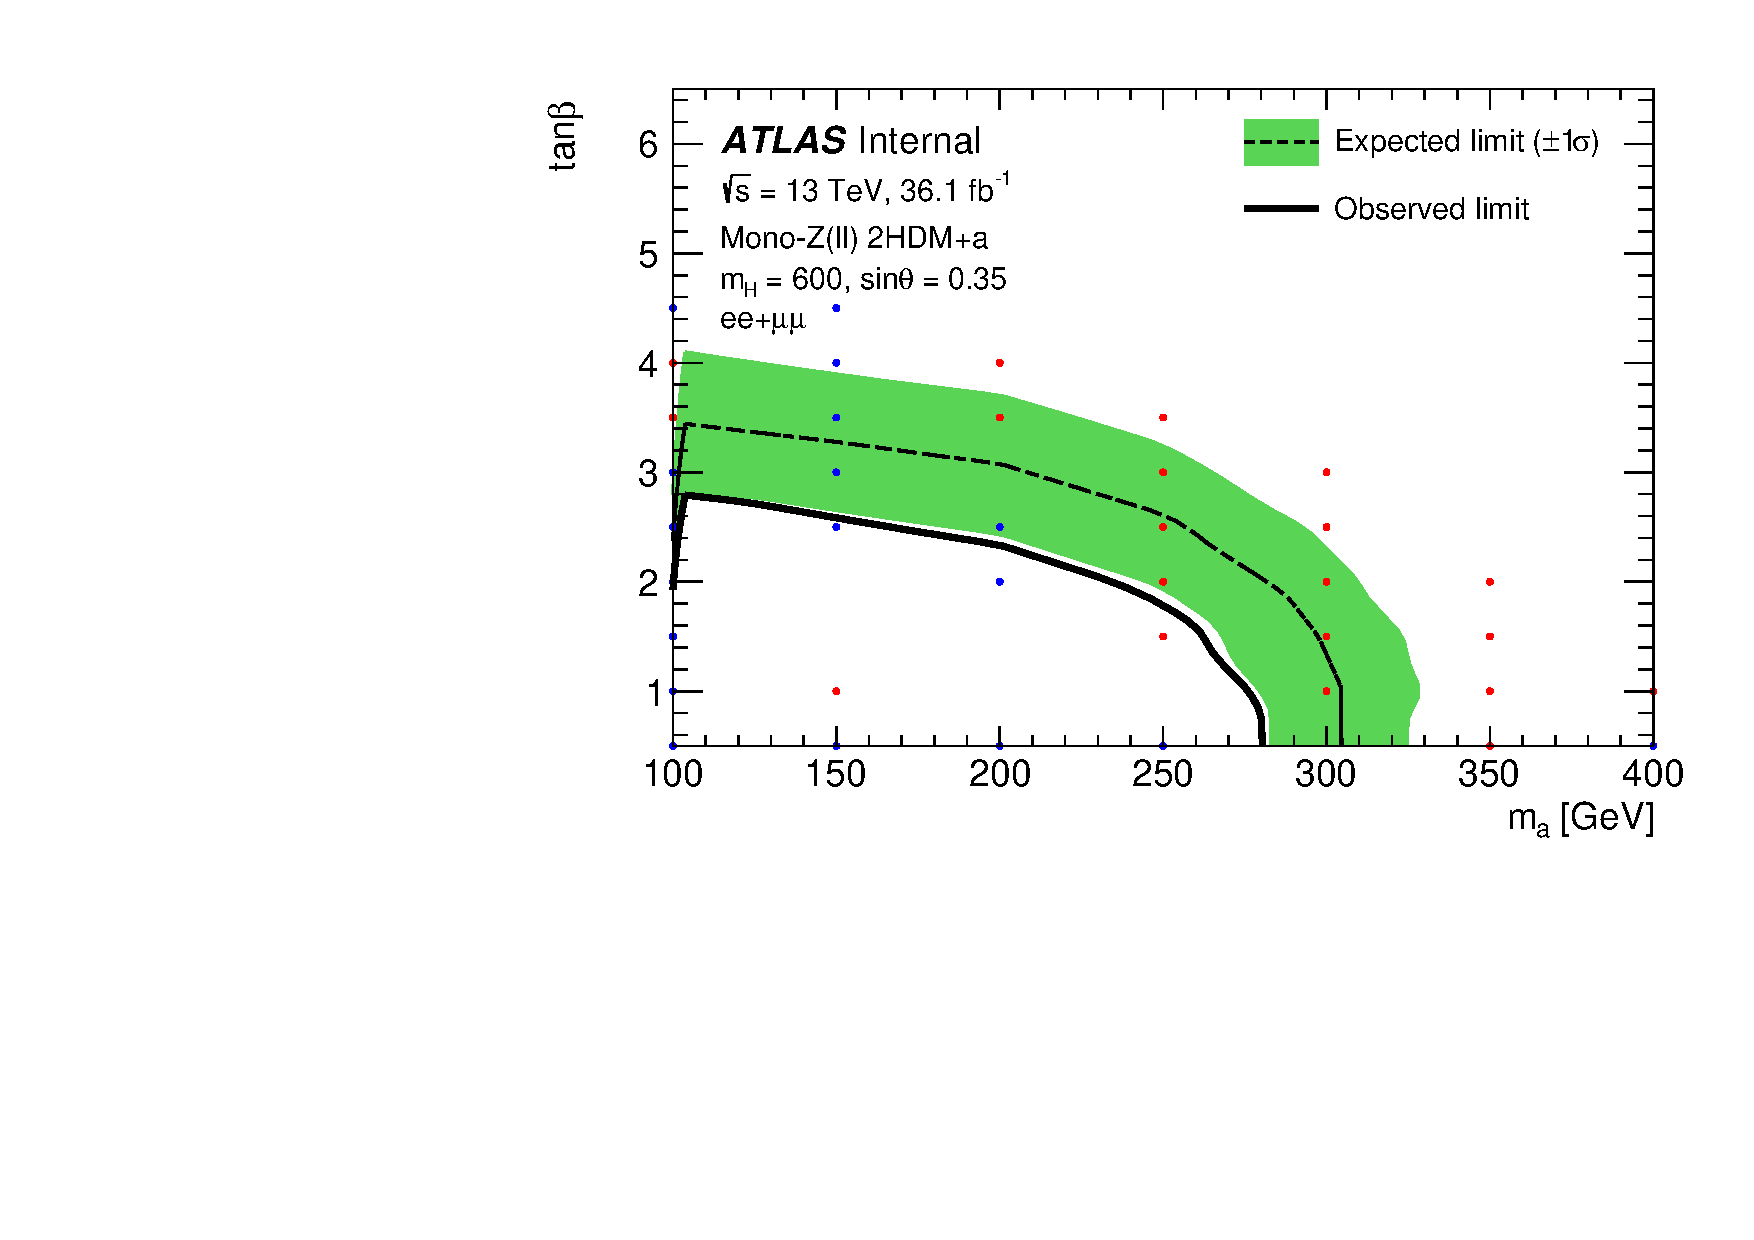
\includegraphics[width=\textwidth]{Figures/limits_2hdma_tan.pdf}
        \label{fig:limits_2hdma_tan}
    \end{subfigure}
    \caption{$m_H$ vs $m_a$ (left) and $\tan(\beta)$ vs $m_a$ (right) exclusion limits with 36.1 \ifb.}
\label{fig:2hdma}
\end{figure}

In the mass limits above, the red points indicate the masses at which there are reconstructed signal samples. The blue points indicate \textit{emulated} points. Mass point emulation is performed to create a finer grid of signal samples without using reconstructed samples. The exclusion contour may look jagged in areas with a coarse grid of signal points. By adding in emulated points, the contour can be made smoother and more physical without going through the tedious process of requesting additional reconstructed MC samples. The method discussed here has been used for the LO simplified models with 36.1 \ifb; emulation for the 2HDM+PS model is more complicated and is not discussed here. 

The validity of emulating signal samples relies on the assumption that the kinematics (i.e. the \etmiss distributions) of the signal does not depend on \mchi in the on-shell region (where $m_\text{med} > 2 m_\chi$). If this is true, then the $E_T^{miss}$ distribution for a reconstructed sample at a given \mmed can be used as the \etmiss distribution for other signal samples with the same \mmed. However, the \etmiss distribution for the emulated sample must be scaled by the ratio of cross sections $\sigma_\text{reco}/\sigma_\text{emul}$. So, as long as the grid of reconstructed points is fine along \mmed, additional points with different \mchi can be emulated just by using the cross sections.

For the axial-vector model, studies on the signal acceptance were been performed and verified that the signal acceptance is flat for a fixed \mmed. For the vector model, an additional complication was that we had a fairly coarse granularity of reconstructed points along \mmed. Because of this, we exploited the similar kinematics between the axial-vector and vector signals and performed emulation from axial-vector $\rightarrow$ vector samples. Emulation for both models has become customary in the \monoZ analysis and will continue to be used moving forward towards the full dataset.


% --------------------------------------------------------------------------------------
\section{Analysis Software}
\label{sec:code}

The MonoZUVic software package is the core of the analysis and has been developed by the UVic group for the past few years. Throughout the evolution of the analysis, contributions have been made towards writing and maintaining the software. The software must be capable of running the entire analysis, including object (electron, muon, jet) calibrations/corrections/selections, removal of overlaps between objects, applying event selections, calculating event weights and kinematic variables, evaluating experimental systematics, and in the end producing trees/histograms for data and MC. Things like calibration recommendations and data formats are in flux quite frequently, and diligent efforts are made to keep the code updated. The software is also cross checked with other groups running the analysis to ensure updated calibrations, squash bugs, etc. The MonoZTruthUVic and MonoZLimitsUVic packages, mentioned briefly above, were written to perform truth-level studies and produce exclusion limits. These packages are also be maintained alongside MonoZUVic. Contributions have also been made to design overhauls in the framework as the analysis has evolved and improved.



